\documentclass{article}
\usepackage[utf8]{inputenc}
\usepackage{graphicx}


\title{\textbf{Concurrent Programming ID1217} \\ 
\textbf{The Gravitational N-body Problem}}
\author{Emil Ståhl}
\date{March 15, 2020}

\begin{document}

\maketitle

\section{Introduction}

This report covers the implementation and evaluation of sequential and parallel programs for a particle computation to solve the gravitational N-body problem. In physics, the n-body problem is the problem of predicting the individual motions of a group of celestial objects interacting with each other gravitationally. Solving this problem has been motivated by the desire to understand the motions of the Sun, Moon, planets, and visible stars. In the 20th century, understanding the dynamics of globular cluster star systems became an important n-body problem. This phenomena can be simulated using different methods, two of which is covered in this work. The first method is generally referred to as the Particle-Particle (PP) method and is using a brute-force technique to simulate the n-body problem. However, due to the O(\(n^2)\) time complexity this method is only suitable for small amounts of particles. But since the method does not approximate the sum its results equals machine precision.\footnote{The Barnes-Hut Algorithm - Tom Ventimiglia and Kevin Wayne} 

To obtain better time complexity some tree methods has been proposed and is widely used in astrophysics. One of which is the Barnes-Hut method that uses an octree to divide the volume into cubic cells and only interactions between particles from nearby cells need to be treated individually; particles in distant cells can be treated collectively as a single large particle centered at the distant cell's center of mass (or as a low-order multipole expansion). This can dramatically reduce the number of particle pair interactions that must be computed. To prevent the simulation from becoming swamped by computing particle-particle interactions, the cells must be refined to smaller cells in denser parts of the simulation which contain many particles per cell. This approximates the result and gives a time complexity of O(n log n) making it feasible for large amounts of particles. 

This report will describe the implementation of both of these methods in a sequential as well as parallel manner. Furthermore, extensive benchmarking and evaluation will be conducted to determine how the methods and implementations differ. The implementation was conducted on a Mac running Mac OS Mojave 10.14.6 and performance was evaluated on HPE ProLiant servers (running Linux) each with 2 x AMD Opteron 6172 (12 cores).

\section{Design and implementation}

This section will describe the implementation of each program.

\subsection{Sequential brute-force}

This program starts in main by taking two arguments from stdin, gnumBodies and numSteps. A new object nBody is then created which initialize a new points array where each entry holds the characteristics of each body. The characteristics include position, velocity, force and mass. When the object is created the main method prints the initial positions of the bodies and then iterates numSteps times and in each iteration invokes the methods \texttt{calculateForces()} that calculates the forces on each body by calculating the distance to the other bodies and \texttt{moveBoodies()} that moves the bodies accordingly. 

\begin{verbatim}
    public void calculateForces() {
    double distance, magnitude, directionX, directionY;

    for (int i = 0; i < gnumBodies; i++) {
        for (int j = i + 1; j < gnumBodies; j++) {
            distance = distance(points[i], points[j]);
            magnitude = (G * points[i].mass * points[j].mass) / (distance * distance);
            directionX = points[j].posX - points[i].posX;
            directionY = points[j].posY - points[i].posY;
            points[i].forceX = points[i].forceX + magnitude * directionX / distance;
            points[j].forceX = points[j].forceX - magnitude * directionX / distance;
            points[i].forceY = points[i].forceY + magnitude * directionY / distance;
            points[j].forceY = points[j].forceY - magnitude * directionY / distance;
        }
      }
    }
\end{verbatim}
This is done sequentially in one thread. When done the final positions of the bodies are printed to stdout. 

\subsection{Parallel brute-force}

The parallel implementation of the brute force algorithm works in a similar way as the sequential program. However, the main method takes in a number of workers as argument to perform the computation in parallel. A new worker class that extends the thread class was created to handle the workers. In main, a new worker object is created for each worker and takes in an id, numSteps, the nBody object as well as a cyclic barrier to be used later. In the worker class a barrier is used to make the threads wait for each other after they have calculated the forces and before they proceed to move the bodies. The barrier used is a part of the java.util.concurrent package where each thread calls barrier.await() to wait for the other threads to arrive. 

The Java run method is similar to how the sequential implementation works where each thread calculates the forces and move the bodies. These two methods are slightly modified to distribute the work among the workers where the outer loop now looks like: \begin{verbatim}
    for (int i = w; i < (int) gnumBodies; i += numWorkers) {
    }
\end{verbatim}{}

By giving each thread an id it is possible to let specific threads do extra work. The printout of the positions is for example handled by the thread with id 0, preventing every thread to print to stdout. 

\subsection{Sequential Barnes-Hut}

As the previous two implementations this program starts by initializing a points array holding the characteristics of each body. However, the implementation is extended with two additional classes, Quad and BHTree. The Quad class represents the space of bodies recursively subdivided into quadrants until each subdivision contains 0 or 1 bodies, some regions do not have bodies in all of their quadrants. The class consists of four methods representing one of the four quadrants along with a boolean method consists() that checks if the specified quadrant contains the given point.  

The BHTree class is where the Barnes-Hut tree is implemented. The class consists of four methods and one of these is insert(Point p) that adds the Point p to the invoking Barnes-Hut tree. If this node does not contain a body, the new Point p is put here. If the node is externel, meaning all four children are null, the region is subdivided further by creating four children. The method then recursively inserts Point p into the appropriate quadrant by invoking the method putBody.

To calculate the force on a body the tree is traversed from the root, this is done in the method updateForce located in the BHTree class. If the center-of-mass of an internal node is sufficiently far from the body, approximate the bodies contained in that part of the tree as a single body, whose position is the group’s center of mass and whose mass is the group’s total mass. The algorithm is fast because we don’t need to individually examine any of the bodies in the group. For external nodes the force is calculated as: 
\begin{verbatim} 
public void addForce(Point p) {         

    double delX = p.posX - this.posX;         
    double delY = p.posY - this.posY;         
    double distance = this.distanceTo(p);                  

    if(distance > 1) {            
    distance = 1;         
    }          
    double force = (G*this.mass*p.mass)/(distance*distance);         
    this.forceX += force*delX/distance;         
    this.forceY += force*delY/distance;     
}
\end{verbatim}
To determine if an internal node is sufficiently far away, the quotient s / d is computed, where s is the width of the region represented by the internal node, and d is the distance between the body and the node’s center-of-mass. Then, this ratio is compared against a threshold value θ. If \(s / d < \Theta\), then the internal node is sufficiently far away and can be calculated with the addForce described above. Else, recurse on each of current node's children.\footnote{The Barnes-Hut Algorithm - Tom Ventimiglia and Kevin Wayne} 

In the main method of the application it iterates numSteps where it each iteration creates a new Quad object and a new tree passing the quad as argument. The gnumBodies is inserted into the tree and then the forces are calculated with the method described above. Lastly, the bodies are moved. When done the final positions are printed to stdout. This is done sequentially in one thread. 

\subsection{Parallel implementation of Barnes-Hut}

To parallelize the program described in chapter 4.3 the main method takes in a number of workers as argument. As in the parallel version of the brute-force algorithm the workers are handled in a separate class Worker. In the worker class the barrier is once again used to wait for threads for finish.  The Java run method handles what was previously done in main i.e. iterate numSteps, creating the tree and calculate forces for assigned points. The barrier is placed between the calculation of forces and the moving of points. When finished the positions are printed to stdout. 

\clearpage
\section{Evaluation}
A test was performed for each program: Each parallel program was evaluated on a different number of threads (1, 2, 3, 4) and a number of different workloads (120, 180, 240). For each (numThreads, workload) the median of at least 5 runs was picked. The results are shown in the graphs below. The complete list of all runs are shown in the appendix.

\subsection{Sequential brute-force}
\begin{verbatim}
#bodies time(s)

120     15.077889627000001
180     33.666206593000005
240     59.629439299000005
\end{verbatim}
\begin{figure}[h]
\centering
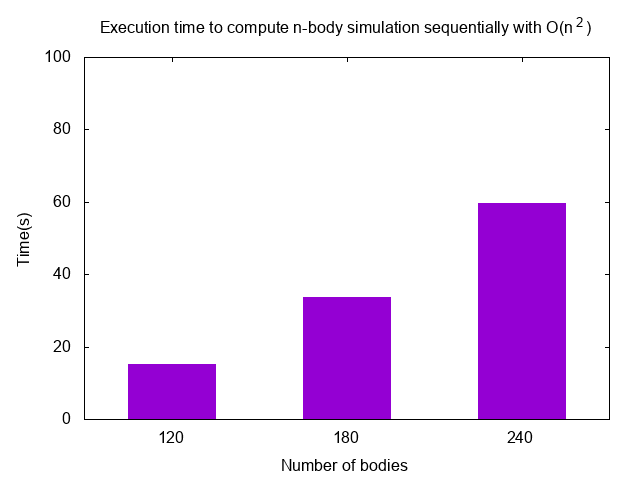
\includegraphics[scale=0.7]{sequential.png}
\caption{Benchmarking of N-body simulation with 56.500 number of steps}
\end{figure}      

\clearpage
\subsection{Parallel brute-force}
\begin{verbatim}
120 bodies

#threads time(s)

1       16.280161247
2       24.733374348
3       14.639581457
4       14.220481049

180 bodies 

#threads time(s)

1       36.322307176  
2       33.985230025  
3       29.416021235
4       26.334773503

240 bodies

#threads time(s)

1       64.341554767 
2       92.661134272 
3       50.14053348 
4       44.190347251
\end{verbatim}
\begin{figure}[h]
\centering
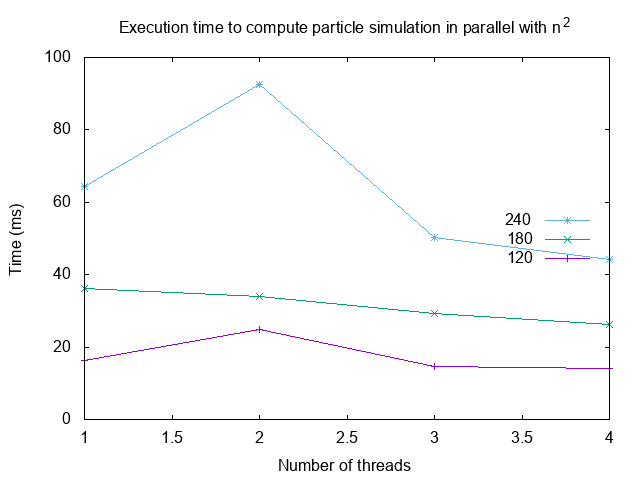
\includegraphics[scale=0.7]{parallel.png}
\caption{Benchmarking of N-body simulation with 56.500 number of steps}
\end{figure}      

\clearpage
\subsection{Sequential Barnes-Hut}
\begin{verbatim}
#bodies time(s)

120     14.449
180     14.255
240     14.534
\end{verbatim}
\begin{figure}[h]
\centering
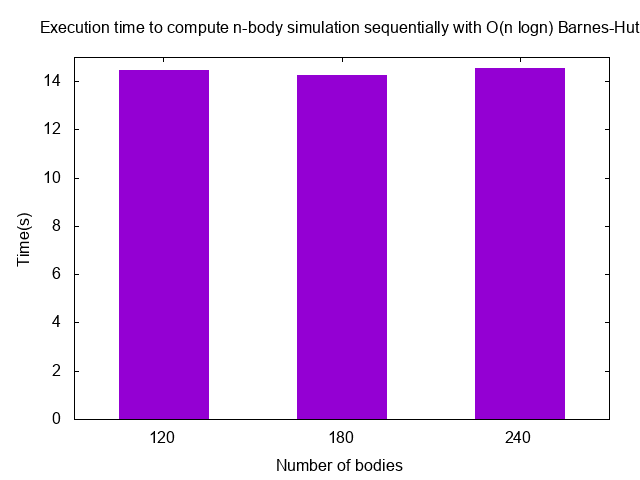
\includegraphics[scale=0.7]{BH-sequential.png}
\caption{Benchmarking of N-body simulation with 56.500 number of steps}
\end{figure}      
\clearpage

\subsection{Parallel Barnes-Hut}
\begin{verbatim}
120 bodies

#threads time(s)

1       1.930
2       2.770
3       3.427
4       3.912

180 bodies

#threads time(s)

1       2.420
2       3.323
3       3.855
4       4.295

240 bodies

#threads time(s)

1       3.633
2       4.042
3       4.914
4       5.078
\end{verbatim}
\begin{figure}[h]
\centering
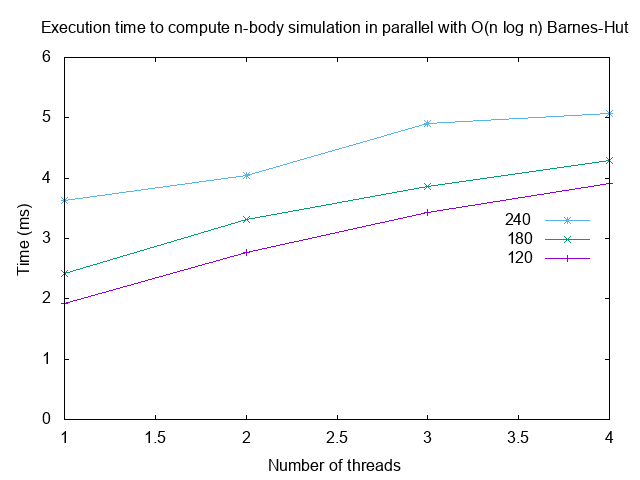
\includegraphics[scale=0.48]{BH-parallel.png}
\caption{Benchmarking of N-body simulation with 56.500 number of steps}
\end{figure}

\subsection{Explanation of results}
When looking on the benchmarks of the sequential brute-force implementation the results are as expected were the execution time rises with the number of bodies. When comparing this to the parallel brute-force there can be noticed that the sequential is faster on 120 bodies compared to the parallel executing with one thread This is probably due to the overhead of creating threads. However, when running on three and four threads the parallel is faster than the sequential implementation. This is probably due to the overhead of creating several threads is negligible compared to the gains in performance when running on multiple threads. The same phenomena can be found when evaluating the performance on 180 as well as 240 bodies executed sequentially and in parallel. 

Regarding the sequential Barnes-Hut implementation there is a very large improvement in performance (~3.1x) compared to the brute-force algorithm. This is because the Barnes-Hut method approximates the forces making it a lot faster but also less accurate compared to the brute-force method.   

Lastly, when evaluating the parallel implementation of the Barnes-Hut algorithm there can be noticed that this is the by far the most efficient implementation where it shows an increase of 4x in performance compared to the sequential Barnes-Hut on 240 bodies. The difference is even bigger when comparing to the sequential brute-force were the increase is ~16,5x. However, the execution time seems to increase with the number of threads. There is no sure explanation for this but it may be due to the overhead of creating threads compared to the already low execution time, which results in that the time spent on creating thread becomes a bigger fraction of the execution time. But this may change as the workload increases, i.e. the overhead gets negligible compared to the gains in performance. Further research could preferably examine this. 



\section{Conclusions}

This paper has covered the implementation of sequential and parallel programs of the Gravitational N-body Problem. Two methods were used were the first is a brute-force algorithm running in O(\(n^2)\) and an approximating method that runs in O(n log n). The evaluation of the different implementations shows that the parallel versions is by far the most efficient but there is some overhead of creating new threads, this overhead is negligible when executing with more threads or larger data sets. This work has provided a deeper understanding of concurrent programming as well as an introduction to the Gravitational N-body Problem. 

\end{document}